\begin{appendices}
    
\section{\sne~magnitude}

\begin{figure}[htbp]
\begin{center}
  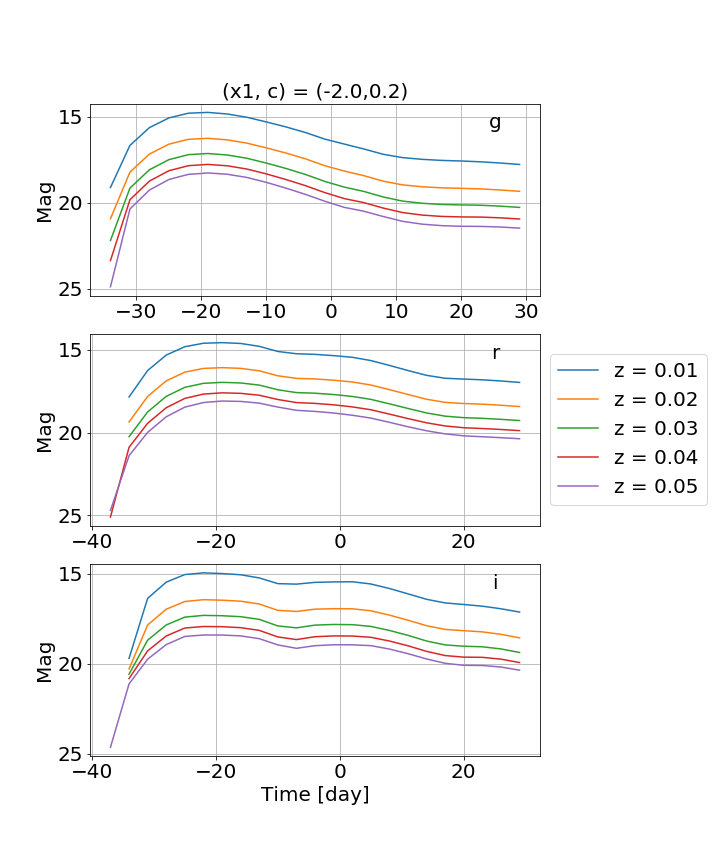
\includegraphics[width=0.9\textwidth]{LC_faint.png}
 \caption{Magnitude as a function of time and redshift for a faint type Ia supernovae and for g (top), r(middle) and i (bottom) bands.}\label{fig:lcfaint}
\end{center}
\end{figure}

\begin{figure}[htbp]
\begin{center}
  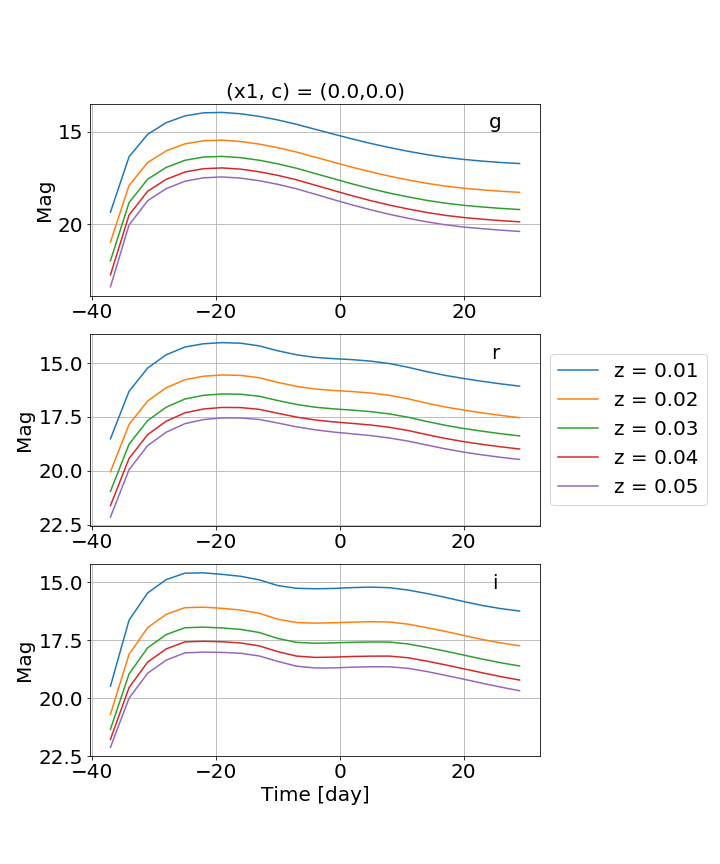
\includegraphics[width=0.9\textwidth]{LC_medium.png}
 \caption{Magnitude as a function of time and redshift for a medium type Ia supernovae and for g (top), r(middle) and i (bottom) bands.}\label{fig:lcmedium}
\end{center}
\end{figure}

\begin{figure}[htbp]
\begin{center}
  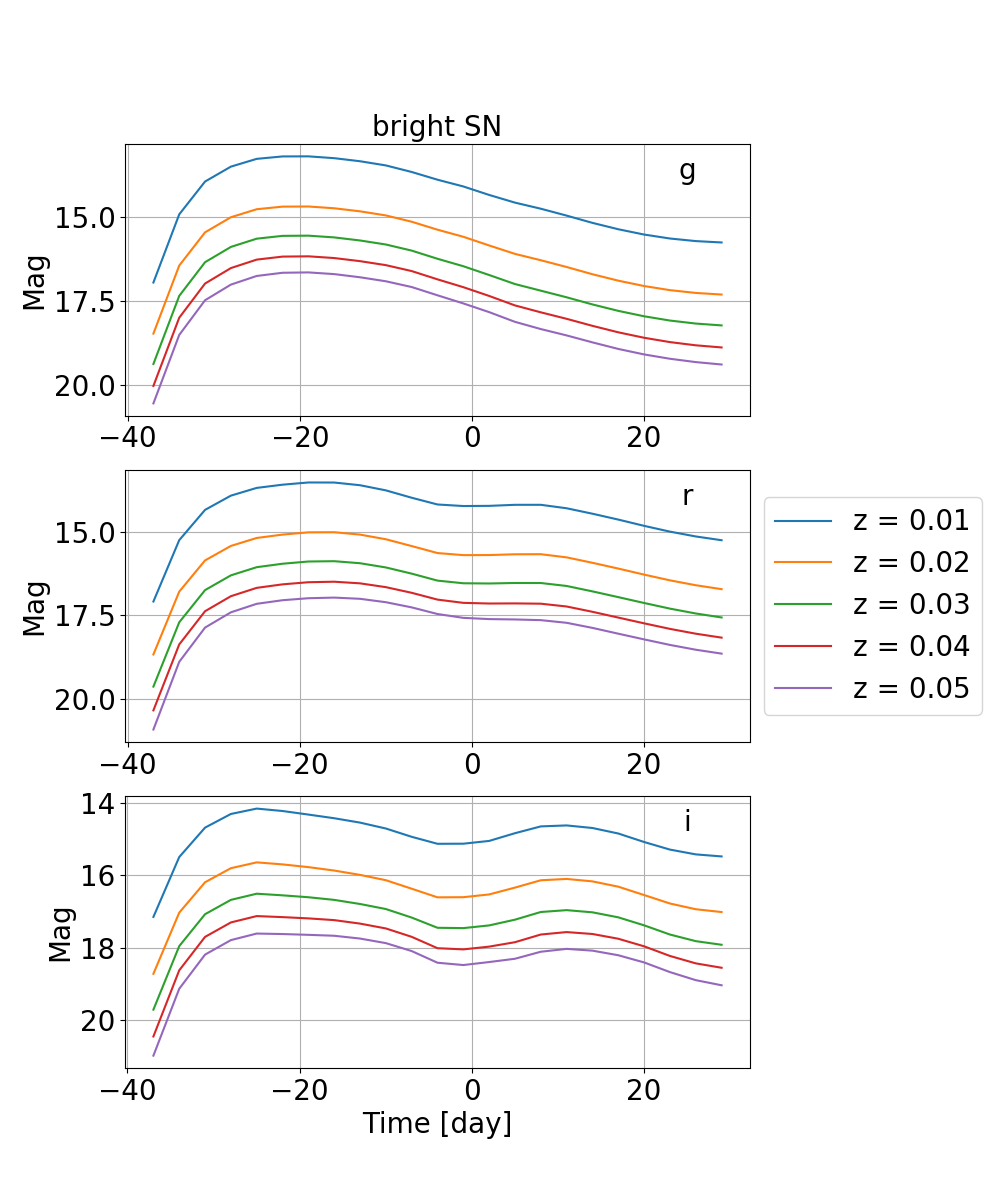
\includegraphics[width=0.9\textwidth]{LC_bright.png}
 \caption{Magnitude as a function of time and redshift for a bright type Ia supernovae and for g (top), r(middle) and i (bottom) bands.}\label{fig:lcbright}
\end{center}
\end{figure}

\begin{figure}[htbp]
\begin{center}
  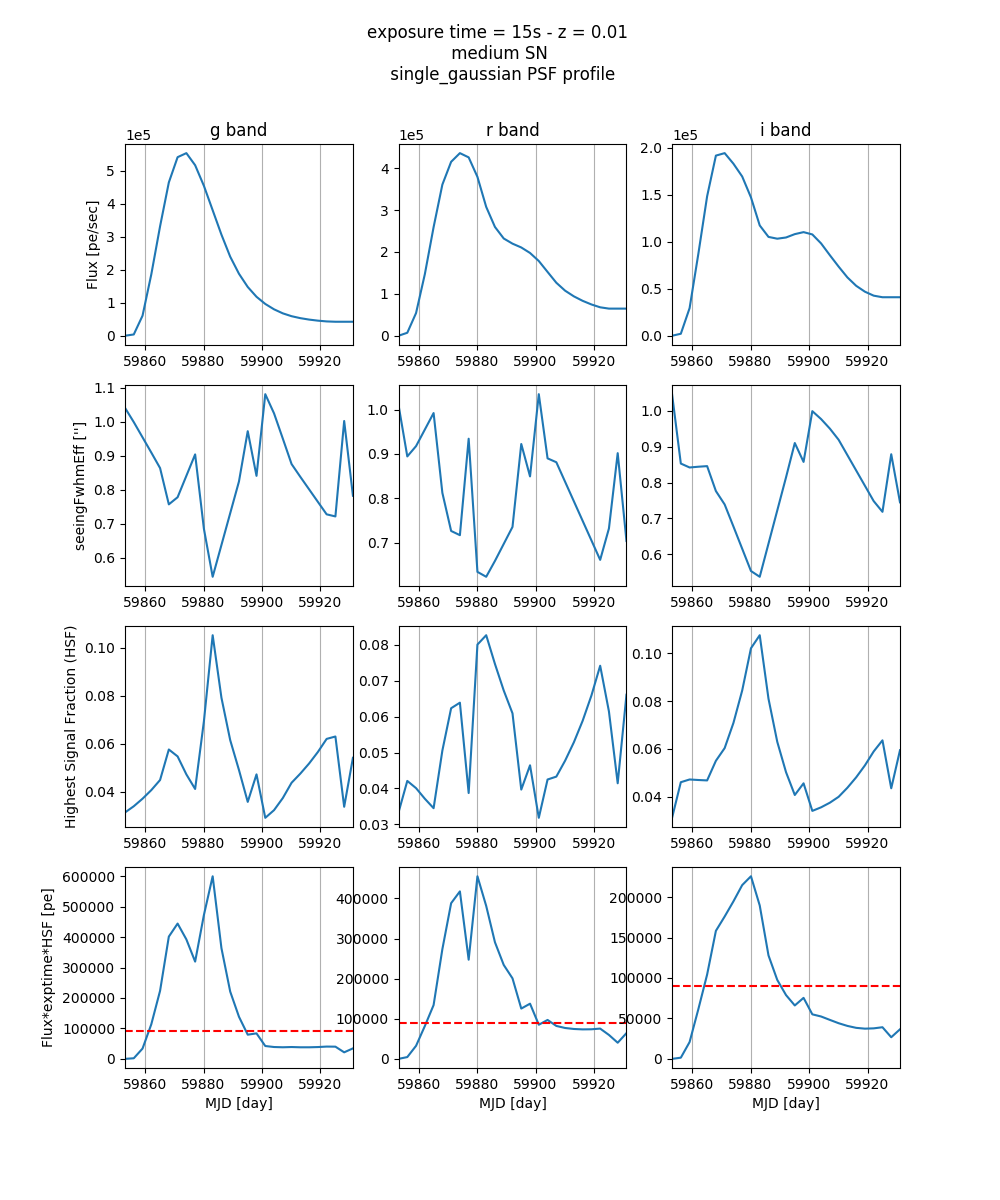
\includegraphics[width=0.9\textwidth]{procedure.png}
 \caption{Illustration of the method used to estimate saturation Effects. To each LC simulated point (first row) corresponds a seeing (second row) from which a factor corresponding to the highest fraction of energy deposited in a pixel is estimated (third row). We multiply this factor by the exposure time (here 15s) and the flux to estimate (fourth row) the highest signal deposited (in pe) in a pixel. A comparison with a chosen full well (red dotted line; 90 kpe) enables us to remove LC points corresponding to saturation.}\label{fig:method}
\end{center}
\end{figure}


\end{appendices}
